%%%%%%%%%%%%%%%%%%%%%%%%%%%%%%%%%%%%%%%%%%%%%%%%%%%%%%%%%%%%%%%%%%%%%%%%%%%%%%%%
\section{A first Workflow}

%%%%%%%%%%%%%%%%%%%%%%%%%%%%%%%%%%%%%%%%%%%%%%%%%%%%%%%%%%%%%%%%%%%%%%%%%%%%%%%%
\begin{frame}
    \frametitle{Outline}
    \begin{columns}[t]
        \begin{column}{.5\textwidth}
            \tableofcontents[sections={1-9},currentsection]
        \end{column}
        \begin{column}{.5\textwidth}
            \tableofcontents[sections={10-18},currentsection]
        \end{column}
    \end{columns}
\end{frame}

%%%%%%%%%%%%%%%%%%%%%%%%%%%%%%%%%%%%%%%%%%%%%%%%%%%%%%%%%%%%%%%%%%%%%%%%%%%%%%%%
\begin{frame}
  \frametitle{What is this about?}
   \question[Questions]{How do I write a simple workflow?}
   \docs[Objectives]{\begin{enumerate}
                      \item Understand the components of a Snakefile: rules, inputs, outputs, and actions.
                      \item Write a simple Snakefile.
                      \item Run Snakemake from the shell.
                     \end{enumerate}}
\end{frame}


%%%%%%%%%%%%%%%%%%%%%%%%%%%%%%%%%%%%%%%%%%%%%%%%%%%%%%%%%%%%%%%%%%%%%%%%%%%%%%%%
\subsection{A first Rule}


%%%%%%%%%%%%%%%%%%%%%%%%%%%%%%%%%%%%%%%%%%%%%%%%%%%%%%%%%%%%%%%%%%%%%%%%%%%%%%%%
\begin{frame}[fragile]
  \frametitle{Layout of a Workflow Development Directory} 
  \task{We are going to work in the \texttt{zipf\_analysis}-folder. Please \texttt{cd} there.}
  \pause
  The idea is to have a neat overview:
  \begin{columns}
    \begin{column}{0.5\textwidth}
      
  \begin{minipage}[t]{0.5\textwidth}
    \setstretch{0.1}
            {\tiny \DTsetlength{0.2em}{1em}{0.2em}{0.4pt}{.6pt}
\dirtree{%
.1 {\textit{workflow\ folder}}.
.2 {scripts}.
.3 {some\ scriptfile.py}.
.3 {some\ scriptfile.sh}.
.3 {some\ scriptfile.R}.
.2 {Snakefile}.
.2 {and more \ldots}.
}}
    \end{minipage}
    \end{column}
    \begin{column}{0.5\textwidth}
      \hint{Our long term goal:\newline Have a orderly overview and seperation of data and code.}
      \pause 
      \question{Any idea why?}
    \end{column}


  \end{columns}

  
\end{frame}


%%%%%%%%%%%%%%%%%%%%%%%%%%%%%%%%%%%%%%%%%%%%%%%%%%%%%%%%%%%%%%%%%%%%%%%%%%%%%%%%
\begin{frame}[fragile]
  \frametitle{Our first \texttt{Snakefile}!}
  \begin{onlyenv}<1| handout:1>
    Create a file, called \texttt{Snakefile}, with no file extension and containing the following content:
    \begin{lstlisting}[language=Python,style=Python]
# Count words.
rule count_words:
    input:    '../books/isles.txt'
    output:   'isles.dat'
    shell:    'python scripts/wordcount.py' 
               ' -i ../books/isles.txt-o isles.dat'
    \end{lstlisting}

  This is a build file, which for Snakemake is called a Snakefile — a file executed by Snakemake. Note that aside from a few keyword additions like \texttt{rule}, it follows standard Python 3 syntax.
  \hint{Stick with \texttt{geany} as the editor.}
    \end{onlyenv}
  \begin{onlyenv}<2| handout:0>
   Now, let's have a detailed look:
   \begin{lstlisting}[language=Python,style=Python]
# Count words.
rule count_words:
    input:    '../books/isles.txt'
    output:   'isles.dat'
    shell:    'python scripts/wordcount.py' 
               ' -i ../books/isles.txt-o isles.dat'
    \end{lstlisting}
    The \texttt{\#} denotes a comment. Any text from \texttt{\#} to the end of the line is ignored by Snakemake.
  \end{onlyenv}
  \begin{onlyenv}<3| handout:0>
   Now, let's have a detailed look:
   \begin{lstlisting}[language=Python,style=Python]
# Count words.
rule count_words:
    input:    '../books/isles.txt'
    output:   'isles.dat'
    shell:    'python scripts/wordcount.py' 
               ' -i ../books/isles.txt-o isles.dat'
    \end{lstlisting}
    \texttt{isles.dat} is a \emph{target}, a file to be created, or built. In Snakemake, these are called “outputs”, for simplicity’s sake.
  \end{onlyenv}
  \begin{onlyenv}<4| handout:0>
   Now, let's have a detailed look:
   \begin{lstlisting}[language=Python,style=Python]
# Count words.
rule count_words:
    input:    '../books/isles.txt'
    output:   'isles.dat'
    shell:    'python scripts/wordcount.py' 
               ' -i ../books/isles.txt-o isles.dat'
    \end{lstlisting}
    \texttt{../books/isles.txt} is a \emph{dependency}, a file that is needed to build or update the target. Targets can have zero or more dependencies. Dependencies in Snakemake are called “inputs”.
  \end{onlyenv}
  \begin{onlyenv}<5| handout:0>
   Now, let's have a detailed look:
   \begin{lstlisting}[language=Python,style=Python]
# Count words.
rule count_words:
    input:    '../books/isles.txt'
    output:   'isles.dat'
    shell:    'python scripts/wordcount.py' 
               ' -i ../books/isles.txt-o isles.dat'
    \end{lstlisting}
    The Python-Command is an \emph{action}, a command to run to build or update the target using the dependencies. In this case the action is a set of shell commands (we can also use Python code… more on that later).
  \end{onlyenv}
  \begin{onlyenv}<6| handout:0>
  Also:
  \begin{enumerate}
   \item Like Python, you can use either tabs or spaces for indentation — don’t use both!
   \item Together, the target, dependencies, and actions form a rule. A rule is a recipe for how to make things.
   \item It does not matter that the shell-command is multi-line. However, pay attention to the leading space in the $2^\mathsf{nd}$ line.
  \end{enumerate}
  \end{onlyenv}
\end{frame}

%%%%%%%%%%%%%%%%%%%%%%%%%%%%%%%%%%%%%%%%%%%%%%%%%%%%%%%%%%%%%%%%%%%%%%%%%%%%%%%%
\begin{frame}[fragile]
  \frametitle{Finally - Running \texttt{Snakemake}!}
  Now, we can run \texttt{Snakemake}:
  \begin{lstlisting}[language=Bash, style=Shell]
$ snakemake --cores=1
  \end{lstlisting}
  \hint[Note:]{The \texttt{-\,-cores=1} is necessary, because we are executing ``locally'' and \texttt{Snakemake} would like to know how much of the resources we may use (you can try without, though, to see what happens.}
  You should see the expected output (\texttt{ls}) and lines which reads:
  \begin{lstlisting}[style=Plain, basicstyle=\footnotesize]
1 of 1 steps (100%) done
Complete log: .snakemake/log/2022-09-17T145657.968906.snakemake.log
  \end{lstlisting}
\end{frame}

%%%%%%%%%%%%%%%%%%%%%%%%%%%%%%%%%%%%%%%%%%%%%%%%%%%%%%%%%%%%%%%%%%%%%%%%%%%%%%%%
\begin{frame}[fragile]
  \frametitle{Re-Running Workflows}
  Try to run \texttt{Snakemake} again:
  \begin{lstlisting}[language=Bash, style=Shell]
$ snakemake --cores=1
  \end{lstlisting}
  \pause
  Oops:
  \begin{lstlisting}[style=Plain, basicstyle=\footnotesize]
Nothing to be done (all requested files are present and up to date).
  \end{lstlisting}
  \pause
  Now, do:
  \begin{lstlisting}[language=Bash, style=Shell]
$ touch ../books/isles.txt
$ ls -l ../* # will proove: the input is more 
          # recent the the output
  \end{lstlisting}
  And run \texttt{Snakemake} once more.
  \question{What happens? Why?}
\end{frame}

%%%%%%%%%%%%%%%%%%%%%%%%%%%%%%%%%%%%%%%%%%%%%%%%%%%%%%%%%%%%%%%%%%%%%%%%%%%%%%%%
\begin{frame}
  \frametitle{When do Rules get executed? - The Solution}
  When it is asked to build a target, \texttt{Snakemake} checks the “last modification time” of both the \emph{target} and its \emph{dependencies}.
  If either
  \begin{itemize}
   \item any dependency has been updated
   \item or a job failed to produce a target (completely)
  \end{itemize}
  upon re-run \texttt{Snakemake} will only rebuild the files that, either directly or indirectly, depend on the file that changed. This is called an \emph{incremental build}.
  \pause
  \docs{By explicitly recording the inputs to and outputs from steps in our analysis and the dependencies between files, Snakefiles act as a type of documentation, reducing the number of things we have to remember.}
\end{frame}

%%%%%%%%%%%%%%%%%%%%%%%%%%%%%%%%%%%%%%%%%%%%%%%%%%%%%%%%%%%%%%%%%%%%%%%%%%%%%%%%
\begin{frame}[fragile]
  \frametitle{Proceeding naively}
  Let’s add another rule to the end of \texttt{Snakefile}. Note that rules cannot have the same name, so we’ll call this one \texttt{count\_words\_abyss}.
  \begin{lstlisting}[language=Python,style=Python]
rule count_words_abyss:
    input:    '../books/abyss.txt'
    output:   'abyss.dat'
    shell:    'python scripts/wordcount.py' 
               ' -i ../books/abyss.txt -o abyss.dat'
  \end{lstlisting}
  \task{Run \texttt{Snakemake} - what happens?}
\end{frame}

%%%%%%%%%%%%%%%%%%%%%%%%%%%%%%%%%%%%%%%%%%%%%%%%%%%%%%%%%%%%%%%%%%%%%%%%%%%%%%%%
\begin{frame}[fragile]
  \frametitle{Rules need targets!}
  Nothing happens because \texttt{Snakemake} attempts to build the first target it finds in the Snakefile, the default target, which is \texttt{isles.dat} which is already up-to-date. We need to explicitly tell \texttt{Snakemake} we want to build \texttt{abyss.dat}:
  \begin{lstlisting}[language=Bash, style=Shell]
$ snakemake --cores=1 abyss.dat
  \end{lstlisting}
\end{frame}

%%%%%%%%%%%%%%%%%%%%%%%%%%%%%%%%%%%%%%%%%%%%%%%%%%%%%%%%%%%%%%%%%%%%%%%%%%%%%%%%
\begin{frame}[fragile]
  \frametitle{``Up to Date'' Versus ``Nothing to be Done''}
  If we ask \texttt{Snakemake} to build a file that already exists and is up to date, then \texttt{Snakemake} informs us that:
  \begin{lstlisting}[style=Plain]
Nothing to be done
  \end{lstlisting}
  \pause
  If we ask \texttt{Snakemake} to build a file that exists but for which there is no rule in our Snakefile, then we get a message like:
  \begin{lstlisting}[language=Bash, style=Shell, basicstyle=\footnotesize]
$ snakemake wordcount.py
# skipping some output
MissingRuleException:
No rule to produce wordcount.py (if you use input functions make sure
that they don't raise unexpected exceptions).
  \end{lstlisting}
  \hint{When we see this error, double-check that you have a rule to produce that file, and also that the filename has been specified correctly. Even a small difference in a filename will result in a \texttt{MissingRuleException}.}
\end{frame}

%%%%%%%%%%%%%%%%%%%%%%%%%%%%%%%%%%%%%%%%%%%%%%%%%%%%%%%%%%%%%%%%%%%%%%%%%%%%%%%%
\begin{frame}[fragile]
  \frametitle{Rules without Outputs?!}
  We may want to remove all our data files so we can explicitly recreate them all. We can introduce a new target, and associated rule, to do this. We will call it clean, as this is a common name for rules that delete auto-generated files, like our \texttt{.dat} files:
  \begin{lstlisting}[language=Python,style=Python]
rule clean:
    shell: 'rm -f *.dat'
  \end{lstlisting}
  There are no in- or outputs! When we invoke the rule, 
  \begin{lstlisting}[language=Bash, style=Shell]
$ snakemake --cores=1 clean
  \end{lstlisting}
  our  \texttt{.dat} files are deleted.
\end{frame}

%%%%%%%%%%%%%%%%%%%%%%%%%%%%%%%%%%%%%%%%%%%%%%%%%%%%%%%%%%%%%%%%%%%%%%%%%%%%%%%%
\begin{frame}[fragile]
  \frametitle{Rules without Outputs?! - II }
  We can add a similar command to create all the data files. We can put this \textbf{at the top} of our Snakefile so that it is the default target, which is executed by default if no target is given to the snakemake command:
  \begin{lstlisting}[language=Python,style=Python]
rule dats:
    input:
        'isles.dat'@,@
        'abyss.dat'
  \end{lstlisting}
  This rule is also an example of a rule that has no actions. It is used purely to trigger the build of its dependencies, if needed.

  If we run,
  \begin{lstlisting}[language=Bash, style=Shell] 
$ snakemake --cores=1 dats
  \end{lstlisting}
  \texttt{Snakemake} creates those files.
\end{frame}

%%%%%%%%%%%%%%%%%%%%%%%%%%%%%%%%%%%%%%%%%%%%%%%%%%%%%%%%%%%%%%%%%%%%%%%%%%%%%%%%
\begin{frame}[fragile]
  \frametitle{Dependencies form a DAG!}
  \begin{exampleblock}{Dependencies}
    The order of rebuilding dependencies is arbitrary. You should not assume that they will be built in the order in which they are listed.
    Dependencies must form a directed acyclic graph (DAG). A target cannot depend on a dependency which itself, or one of its dependencies, depends on that target.
  \end{exampleblock}
  If we run dats again, then snakemake will see that the dependencies (\texttt{isles.dat} and \texttt{abyss.dat}) are already up to date. Given the target dats has no actions, there is nothing to be done:
  \begin{lstlisting}[language=Bash, style=Shell] 
$ snakemake --cores=1 dats
# ...
Nothing to be done
  \end{lstlisting}
\end{frame}

%%%%%%%%%%%%%%%%%%%%%%%%%%%%%%%%%%%%%%%%%%%%%%%%%%%%%%%%%%%%%%%%%%%%%%%%%%%%%%%%
\begin{frame}[fragile]
  \frametitle{What do we have - UP TO NOW?}
  \begin{columns}
   \begin{column}{0.8\textwidth}
     Our ``Workflow'' so far:
     \begin{lstlisting}[language=Python,style=Python, basicstyle=\tiny]
rule dats:
     input:
         'isles.dat',
         'abyss.dat'

# delete everything so we can re-run things
rule clean:
    shell: 'rm -f *.dat'

# count words in one of our "books"
rule count_words:
    input:    'books/isles.txt'
    output:   'isles.dat'
    shell:    'python scripts/wordcount.py'
              ' -i books/isles.txt -o isles.dat'

rule count_words_abyss:
    input:    'books/abyss.txt'
    output:   'abyss.dat'
    shell:    'python scripts/wordcount.py' 
              ' -i books/abyss.txt -o abyss.dat'     
     \end{lstlisting}

   \end{column}
   
   \begin{column}{0.2\textwidth}
     The DAG can be graphed like this:
     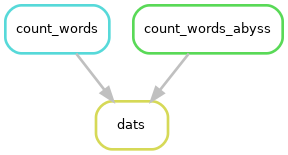
\includegraphics[width=\textwidth]{workflows/mini_dag.png}
     2 producers, a single target rule.
   \end{column}
  \end{columns}
\end{frame}

%%%%%%%%%%%%%%%%%%%%%%%%%%%%%%%%%%%%%%%%%%%%%%%%%%%%%%%%%%%%%%%%%%%%%%%%%%%%%%%%
\begin{frame}[fragile]
  \frametitle{\HandsOn{Add some Stuff!}}
  \begin{enumerate}
   \item Write a new rule for last.dat, created from \texttt{books/last.txt}.
   \item Update the \texttt{dats} rule with this target.
   \item Write a new rule for \texttt{results.txt}, which creates the summary table. The rule needs to:
        \begin{itemize}
         \item Depend upon each of the three .dat files.
         \item Invoke the action \texttt{python scripts/zipf\_test.py abyss.dat isles.dat last.dat > results.txt}.
        \end{itemize}
   \item Put this rule at the top of the Snakefile so that it is the default target.
   \item Update clean so that it removes results.txt.
  \end{enumerate}
\end{frame}


  

